%!TEX root = main.tex
\section{Overview of The Methodology}
\seclabel{overview}
%
%
%\JW{Fixed: In general, I think this section needs to describe the ACC example (which it does) but also needs to make sure the reviewers know how everything can be generalized.  These insights will segue nicely to the \toolreaffirm discussion in the next section.}
%
In this section, we will explain our methodology through a simplified example of the ACC system. This system has been designed to satisfy safety requirements pertaining to vehicle spacing that varies with vehicle speed.
%
%
%
Assume that a designer has previously modeled the ACC system as a combination of the vehicle dynamics and an ACC module, and GPS measurements were considered trusted in the initial design. In the following, we will describe the ACC system as originally designed, an attack scenario, and an example of resiliency pattern to repair the ACC model\footnote{We note that the ACC model presented herein is not a representative of the complexity of a true ACC system, but a simplified example in which the dynamics and control equations are chosen for simplicity in the ensuing discussion of the paper.}.
%
Then, we present how \toolreaffirm can automatically perform a model transformation and synthesis to construct a new ACC model with resiliency. 
%
%which will (in the subsequent discussion) be adapted to satisfy a resiliency requirement.
% the structure of \toolreaffirm and demonstrate
%

\subsection{A Simplified Example of ACC System}



%To illustrate and motivate our proposed approach, this subsection presents a case study of a control system that aims to safely adapt a vehicle speed, namely, an adaptive cruise control (ACC) system. 

%
%\noindent
%{\bf Original ACC Model.}
%\JW{Fixed: I think we need to acknowledge -- possibly within the subsection title -- that this is a toy example.  Reviewers may take issue with our work if they think that we believe the ACC model used herein is representative of the complexity of a true ACC system.}
%
For simplicity, we assume that the designer initially model the ACC system (including vehicle dynamics) as a hybrid system shown in \figref{original}.
% 
The original ACC system operates in two modes: \emph{speed control} and \emph{spacing control}. In speed control, the host car travels at a driver-set speed. In spacing control, the host car aims to maintain a safe distance from the lead car. 
%
The vehicle has two states in which $d$ is the distance to the lead car, and $v$ is the speed of the host vehicle. The ACC system has two sensors that measure its velocity $v$ via noisy wheel encoders, $\venc = v + \nenc$, and a noisy GPS sensor, $\vgps = v+\ngps$, where $\nenc$ and $\ngps$ denote the encoder and GPS noises, respectively. Additionally, the ACC system has a radar sensor that measures the distance to the lead vehicle, $\drad = d+\nrad$.
%
The ACC system decides which mode to use based on the real-time sensor measurements. For example, if the lead car is too close, the controller triggers the transition $g_{sd}$ to switch from speed control to spacing control. Similarly, if the lead car is further away, the ACC system switches from spacing control to speed control by executing the transition $g_{ds}$. 
%
The \emph{safety specification} of the system is specified that $d$ should always be greater than $\dsafe$, where $\dsafe = v + 5$. We will describe the ACC model in more details in~\secref{result}.
%
%The model has four state variables in which where $d$ is the distance between the host car and the lead car, $v$ is the speed of the host car, $\hat{d}$ and $\hat{v}$ denote the estimated distance and velocity of the host car, respectively. 
%The model has four state variables in which where $d$ and $\hat{d}$ are the actual distance and estimated distance between the host car and the lead car, $v$ and $\hat{v}$ represent the actual velocity and estimated velocity of the host car, respectively. 
% 
%
%Additionally, the ACC system has a radar sensor that measures the distance to the lead vehicle, $\drad = d+\nrad$. In this example, we assume that the lead vehicle travel with a constant speed $\vlead$. The transition from speed control to spacing control occurs when the estimate of the distance is less than twice the estimated safe distance, \ie $\hat{d} < 10 + 2\hat{v}$. A similar condition is provided for transitioning from spacing control to speed control, \ie $\hat{d} \geq 10 + 2\hat{v}$.  The \emph{safety specification} of the system is specified that $d$ should always be greater than $\dsafe$, where $\dsafe = v + 5$.
%
%
%\JW{Fixed: This subsection needs to be short (like it is) but it also needs to let the reviewers know that we agree the model is simple.  Please take another attempt at it -- then I will do a pass to appease people that know something about real-world CPS modeling.}
%
\begin{figure}[t!]%
	\centering%
    %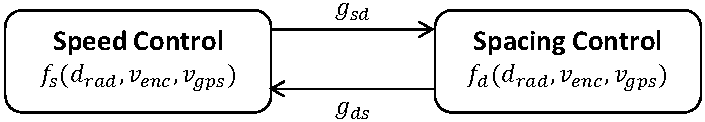
\includegraphics[width=0.48\textwidth]{image/acc_abstract_model}%
		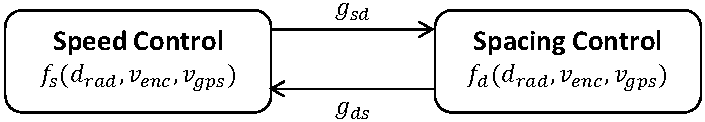
\includegraphics[width=0.46\textwidth]{image/acc_abstract_model}%
		%\includegraphics[trim = 17mm 85mm 17mm 0mm, clip, width=0.95\textwidth]{image/spectral_signal}%
		\vspace{-0.5em}
	\caption{An original ACC model.}%
	\figlabel{original}%
	\vspace{-1em}
\end{figure}%
\begin{figure}[t!]%
	\centering%
    %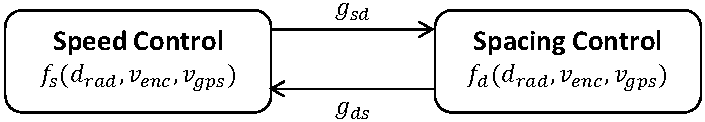
\includegraphics[width=0.48\textwidth]{image/acc_abstract_model}%
		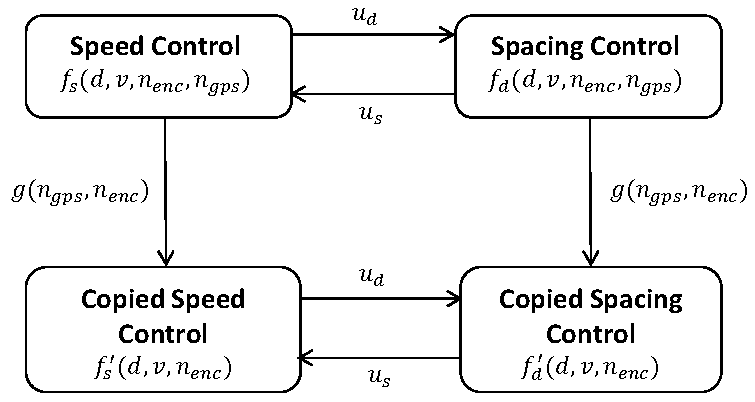
\includegraphics[width=0.48\textwidth]{image/acc_abstract_model_pat1}%
		%\includegraphics[trim = 17mm 85mm 17mm 0mm, clip, width=0.95\textwidth]{image/spectral_signal}%
		\vspace{-0.5em}
	\caption{A repaired ACC model without a reference to GPS sensor under spoofing attacks.}%
	\figlabel{updated}%
	\vspace{-1em}
\end{figure}%

%\subsection{Safety Violation under GPS Sensor Attack}

\vspace{0.5em}
\noindent
{\bf Safety violation under GPS sensor attack.}
%
%
In this example, we assume that after designing and verifying the initial ACC system, it is determined that the GPS sensor can be \emph{spoofed} \cite{tippenhauer2011requirements, kerns2014unmanned}. GPS spoofing occurs when incorrect GPS packets (possibly sent by a malicious attacker) are received by the GPS receiver. In the ACC system, this allows an attacker to arbitrarily change the GPS velocity measurement. 
%
Thus, a new scenario occurs when the original assumption of GPS noise, \eg $|\ngps| \leq 0.05$ is omitted, and the new assumption is $|\ngps| \leq 50$.
As a result, the safety specification could be violated under the GPS sensor attacks, and a designer needs to repair the original model with a resiliency pattern. 




\vspace{0.5em}
\noindent
{\bf Example of resiliency pattern: ignoring GPS measurement.}
%\subsection{Example of Resiliency Pattern}
Since the ACC system has redundancy in the sensory information of its estimated velocity, to provide resilience against the GPS attacks, a mitigation strategy is to ignore the GPS value, and use only the wheel encoders to estimate velocity. 
%
Thus, a potential resiliency pattern is first to create a copy of the original model where the controller simply ignores the GPS reading as it can no longer be trusted. 
%
Then, adding new transitions from the legacy speed and spacing modes of the original model to the new copied speed and spacing modes of the copy that uses only the wheel encoder as a velocity measurement source. We note that this transformation is generic, that is, it can be applied in a uniform manner to any given model simply by creating a duplicate version of each original mode and transition, copying the dynamics in each mode, but without a reference to the variable $\vgps$. 

\figref{updated} illustrates the repaired model in which the transition from the original speeding and spacing control modes to their copies is an expression over $\vgps$ and $\venc$. 
%
Observe that while it would be possible to use only the wheel encoders all the time, a better velocity estimate must be obtained by using an average velocity measurement (from both the GPS and wheel encoders) when the GPS sensor is performing within nominal specifications. The main analysis question is when should the model switch from the original modes to the copied modes during the spoofing attack. %\ie how to determine a transition condition $g(\ngps,\nenc)$. 
%
From a practical standpoint, such a transition should occur when the GPS measurement significantly deviates from the wheel encoder measurement, and a transition condition can be specified as $g(\vgps,\venc) = |\vgps -\venc| \geq \theta$, where $\theta$ is an unknown parameter. 
%
Since $\venc = v + \nenc$ and $\vgps = v+\ngps$, we can rewrite the transition condition as $g(\vgps,\venc) = |\ngps -\nenc| \geq \theta$.
%
Then, one needs to synthesize the suitable value of the parameter $\theta$ that specifies the threshold for switching from the original copy to the new copy so that the safety requirement is satisfied.



\subsection{REAFFIRM Toolkit}
%
Our \toolreaffirm prototype for the model-based design and repair with resiliency is built in Matlab and consists of two main modules, corresponding to a \emph{model transformation} and a \emph{model synthesizer}. To synthesize the model with resiliency to unanticipated attacks, users need to provide the following inputs to \toolreaffirm:
%
\begin{itemize}[leftmargin= 2 em]
    \item the initial design of a hybrid system modeled in MathWorks SLSF format,
		\item the resiliency pattern specified as a model transformation script that transforms the initial model to the new model with resiliency to unanticipated attacks, and
		\item the correctness (safety) requirement of the system specified as an STL formula.
		%\item the specific ranges of unknown parameters whose values need to be synthesized to ensure the STL specification is satisfied. 
%
\end{itemize}

In the case of the ACC example mentioned previously, the inputs of \toolreaffirm are the SLSF model of the original ACC system shown in~\figref{original}, the resiliency pattern that creates the copied version of the original model without a reference to the variable $\vgps$, and the safety requirement encoded as an STL formula 
\begin{align}
\vspace{-1em}
\varphi_{ACC} &= \Box_{[0, \infty)} d[t] < 5 + v[t]. 
\vspace{-1em}
\end{align}
%
The model transformation tool of \toolreaffirm takes the initial SLSF model and the resiliency pattern, and then generates the new SLSF model of the ACC system that contains a parameter $\theta$ captured the switching condition based on the difference between the GPS measurement and the wheel encoder measurement.
%
%
Then, the model synthesizer tool of \toolreaffirm takes the parametrized ACC model in SLSF and the STL formula $\varphi_{ACC}$ as inputs, and then performs a parameter synthesis to find the desired value of $\theta$ over a certain range, to ensure that $\varphi_{ACC}$ is satisfied. Internally, the model synthesizer of \toolreaffirm utilizes an open-source model falsification tool---Breach~\cite{donze2010breach} to synthesize values for the desired parameters. If the synthesizer can find the best value of $\theta$ over the given range, \toolreaffirm outputs a competed SLSF model which satisfies $\varphi_{ACC}$ under the GPS attacks. Otherwise, the tool will suggest a designer to either search over different parameter ranges or try different resiliency patterns to repair the ACC model.   
%

\toolreaffirm was tested using Matlab 2017a and Matlab 2018a executed on an x86-64 laptop with 2.8 GHz Intel(R) Core(TM) i7-7700HQ processor and 32 GB RAM. All performance metrics reported were recorded on this system using Matlab 2018a. In Breach, we choose the CMAES solver, and the maximum optimization time is 30 seconds for each iteration of the falsification loop. \toolreaffirm and all case studies investigated in this paper are available to download at \url{https://github.com/LuanVietNguyen/reaffirm}.

% 
%In the next section, we present the model transformation language that we have developed to assist designers in specifying a resiliency pattern to repair their initial designs effectively.
%Internally, the model synthesizer of \toolreaffirm  utilizes an open-source model falsification tool---Breach~\cite{donze2010breach}, to check an SLSF model against the specification. The counterexamples returned by this falsification tool are used to determine values for the desired parameters. At the end of a falsification loop, the completed model produced by \toolreaffirm, compared to the original model, can have additional modes of operation as well as new transitions between different modes, and as a result, has resilient behaviors specified in the resiliency patterns.   
%
%\begin{itemize}[leftmargin= 2 em]
    %\item \textbf{Model Transformation} takes a given initial model and a resiliency pattern and generates a partial model that contains \emph{holes}, that is, parameters for which values need to be determined to ensure that the correctness requirements are satisfied. The resiliency pattern captures a generic way of transforming models that corresponds to commonly known mitigation strategies. The parameters in the incomplete model correspond to unknown switching conditions, or unknown assignments in variable updates, or even unknown coefficients in controller dynamics. The model is specified using the MathWorks Simulink/Stateflow (SLSF) format, and the correctness requirement is specified in the temporal logic Signal Temporal Logic (STL) that is widely used in tools for verification for cyber-physical systems~\cite{maler2004monitoring}. The resiliency pattern can be specified as a \emph{model transformation script} that operates on the internal representation of SLSF models specifying the desired transformation in a generic way. As an example, for a system that contains a nominal controller and a safety controller, a resiliency pattern can be specified as a transition from a nominal controller to a safety controller.
%%
%\item \textbf{Model Synthesizer} takes a parameterized model (SLSF) and a correctness requirement (STL formula) as inputs and outputs a completed model with parameter values instantiated to satisfy the correctness requirements.  Internally, the tool utilizes an open-source model falsification tool---Breach~\cite{donze2010breach}, to check an SLSF model against the specification. The counterexamples returned by this falsification tool are used to determine values for the desired parameters. At the end of a falsification loop, the completed model produced by \toolreaffirm, compared to the partial behavior model, can have additional modes of operation as well as new transitions between different modes, and as a result, has resilient behaviors specified in the resiliency patterns.
%\end{itemize}
%
%
%
%
%
%

%To provide a resilience for the ACC model, the transformation tool of \toolreaffirm will take the original ACC model shown in ~\figref{original} and the transformation script demonstrated in \figref{examplecode}, and then output the \emph{parameterized} model displayed in \figref{updated}, where the variable $\ngps$ is replaced by the variable $\nenc$ in the resilient speed and spacing control modes, and the value of $\theta$ needs to be determined. Next, the model synthesizer of \toolreaffirm takes the parameterized ACC model, the safety requirement encoded as an STL formula $\Box_{[0, \infty]} (d[t] < 5 + v[t])$, and the specific range of $\theta$, and then calls the synthesizer to determine the best $\theta$ which ensures the final model will always satisfy the safety requirement. 
%

%\begin{figure}[t!]%
	%\centering%
	%\begin{adjustbox}{max size={0.99\columnwidth}{0.75\textheight}}%
	%\begin{tikzpicture}[>=stealth',shorten >=1pt,auto,node distance=8cm,font=\Large]
		%%\tikzstyle{every state}=[minimum size=3cm,font=\normalsize]
		%\tikzstyle{every state}=[font=\Large,rectangle,rounded corners, minimum size=5cm]
		%\node[state] (speed)      			{\makecell[c]{$\textbf{Speed Control}$\\\\
		%$\begin{aligned}
		%\dot{d} & = \vlead - v \nonumber \\
		%\dot{v} & = 2\vlead - v - \hat{v} \nonumber \\
		%\dot{\hat{d}} & = \vlead - \hat{v} + 10(\drad-\hat{d})\nonumber \\
		%\dot{\hat{v}} & = 2\vlead - 3\hat{v} + \frac{1}{2} (\ngps + \nenc) \nonumber\\
		%\end{aligned}$\\\\
		%$\hat{d} \geq 10 + 2\hat{v}$
		%}};
		%\node[state] (space) [right of=speed]	{\makecell[c]{$\textbf{Spacing Control}$\\\\
		%$\begin{aligned}
		%\dot{d} & = \vlead - v \nonumber \\
		%\dot{v} & = 2\vlead - v - \hat{v} -\frac{1}{4}(10 + 2\hat{v}-\hat{d}) \nonumber \\
		%\dot{\hat{d}} & = \vlead - \hat{v} + 10 (\drad-\hat{d})\nonumber \\
		%\dot{\hat{v}} & = 2\vlead - 3\hat{v} + \frac{1}{2} (\ngps + \nenc) -\frac{1}{4}(10 + 2\hat{v}-\hat{d}) \nonumber\\
		%\end{aligned}$\\\\
		%$\hat{d} < 10 + 2\hat{v}$
		%}};
		%
		%\node[state] (res_speed) [below of=speed]  {\makecell[c]{$\textbf{Resilient Speed Control}$\\\\
		%$\begin{aligned}
		%\dot{d} & = \vlead - v \nonumber \\
		%\dot{v} & = 2\vlead - v - \hat{v} \nonumber \\
		%\dot{\hat{d}} & = \vlead - \hat{v} + 10(\drad-\hat{d})\nonumber \\
		%\dot{\hat{v}} & = 2\vlead - 3\hat{v} + \frac{1}{2} (\nenc + \nenc) \nonumber\\
		%\end{aligned}$\\\\
		%$\hat{d} \geq 10 + 2\hat{v}$
		%}};
		%
		%\node[state] (res_space) [right of=res_speed]	{\makecell[c]{$\textbf{Resilient Spacing Control}$\\\\
		%$\begin{aligned}
		%\dot{d} & = \vlead - v \nonumber \\
		%\dot{v} & = 2\vlead - v - \hat{v} -\frac{1}{4}(10 + 2\hat{v}-\hat{d}) \nonumber \\
		%\dot{\hat{d}} & = \vlead - \hat{v} + 10 (\drad-\hat{d})\nonumber \\
		%\dot{\hat{v}} & = 2\vlead - 3\hat{v} + \frac{1}{2} (\nenc + \nenc) -\frac{1}{4}(10 + 2\hat{v}-\hat{d}) \nonumber\\
		%\end{aligned}$\\\\
		%$\hat{d} < 10 + 2\hat{v}$
		%}};
		%
		%
		%\node (speedtospace) [above=6mm of speed,xshift=40mm]{\makecell[c]{$\hat{d} < 10 + 2\hat{v}$}};
		%%$\dot{d} = \vlead - v$\\$\dot{v} = 2\vlead - v - \hat{v} -\frac{1}{4}(10 + 2\hat{v}-\hat{d}$\\$\dot{\hat{d}} = \vlead - \hat{v} + 10(\drad-\hat{d})$\\$\dot{\hat{v}} = 2\vlead - 3\hat{v} + \frac{1}{2} (\ngps + \nenc) -\frac{1}{4}(10 + 2\hat{v}-\hat{d}$}}; 
		%
		%\node[coordinate] (c1) [above=5mm of speed.north] {};
		%\node[coordinate] (c2) [above=5mm of space.north] {};
		%\draw[->]			(speed.north) -- (c1) -- (c2) to (space.north);
		%
		%\node (spacetospeed) [below=6mm of space,xshift=-40mm]{\makecell[c]{$\hat{d} \geq 10 + 2\hat{v}$}};
%
		%\node[coordinate] (c3) [below=5mm of space.south] {};
		%\node[coordinate] (c4) [below=5mm of speed.south] {};
		%\draw[->]			(space.south) -- (c3) -- (c4) to (speed.south);
		%
		%\node (res_speedtospace) [above=6mm of res_speed,xshift=40mm]{\makecell[c]{$\hat{d} < 10 + 2\hat{v}$}};
		%%$\dot{d} = \vlead - v$\\$\dot{v} = 2\vlead - v - \hat{v} -\frac{1}{4}(10 + 2\hat{v}-\hat{d}$\\$\dot{\hat{d}} = \vlead - \hat{v} + 10(\drad-\hat{d})$\\$\dot{\hat{v}} = 2\vlead - 3\hat{v} + \frac{1}{2} (\ngps + \nenc) -\frac{1}{4}(10 + 2\hat{v}-\hat{d}$}}; 
		%
		%\node[coordinate] (c5) [above=5mm of res_speed.north] {};
		%\node[coordinate] (c6) [above=5mm of res_space.north] {};
		%\draw[->]			(res_speed.north) -- (c5) -- (c6) to (res_space.north);
		%
		%\node (res_spacetospeed) [below=6mm of res_space,xshift=-40mm]{\makecell[c]{$\hat{d} \geq 10 + 2\hat{v}$}};
%
		%\node[coordinate] (c7) [below=5mm of res_space.south] {};
		%\node[coordinate] (c8) [below=5mm of res_speed.south] {};
		%\draw[->]			(res_space.south) -- (c7) -- (c8) to (res_speed.south);
		%
		%\node[coordinate] (c9) 	[left=5mm of speed.south] {};
		%\node[coordinate] (c10) [left=5mm of res_speed.north] {};
		%\node[coordinate] (c11) [right=5mm of space.south] {};
		%\node[coordinate] (c12) [right=5mm of res_space.north] {};
		%
		%%\draw[->]			(speed.south)[right=1mm to (res_speed.north);
		%%\draw[->]			(space.south) to (res_space.north);
		%
		%\path[->]			(c9) edge node[xshift=-29mm]{\makecell[c]{$|\ngps -\nenc| \geq \theta$}}(c10); 
		%\path[->]			(c11) edge node[xshift=1mm]{\makecell[c]{$|\ngps -\nenc| \geq \theta$}} (c12); 
		%
		%%
		%%\path[->]			(speed.north) edge[bend left] node{\makecell[c]{$\mathit{OD} \leq \mathit{OD}_t \wedge t_m \geq t_\text{mOn} $\\$t_m' := 0$}} (space.north); 
		%%\path[->]			(space.south)	edge[bend left] node{\makecell[c]{$\mathit{OD} \geq \mathit{OD}_t \wedge t_m \geq t_\text{mOff} $\\$t_m' := 0$}} (speed.south); 
	%\end{tikzpicture}%
	%\end{adjustbox}%
	%\caption{Updated Resilient ACC model}%
	%\figlabel{updated}%
%\end{figure}

%